\section{Implementation}

\subsection{Data Collection}

There is no historical data for bus arrival times available online, so all the data that I will use to train and test my models has to be manually collected. \\

The following bus routes were chosen to collect data from: 6, 7, 9, 14, 35, 37, 52, 69, 267, 277, 328, 452. Of these routes, the 6, 14, 37, 52 and 69 bus routes are twenty four hour bus routes and the 37, 69, 267 and 277 bus routes do not travel through Zone 1. This allows there to be variety in the travel routes, traffic conditions and times of travel and so the data collected is not heavily biased towards particular areas of London. There is also some overlap in stops between the bus routes, for example the 52 to Victoria and the 452 to Vauxhall have a 23 stop (and therefore, also route) overlap from "Station Terrace" to  "Knightsbridge Station /\ Harrods". This ensures information on journey times between stops doesn't rely on data from just one bus route. \\

\textbf{1) Call Countdown API}: The JSON information returned from the Countdown call is converted into a list of dictionaries, where each dictionary represents a single vehicle. The format of each dictionary is as below:

\begin{lstlisting}
    vehicle_info = {
                "vehicle_id": vehicle_id,
                "bus_stop_id": bus_stop_id,
                "direction": direction,
                "expected_arrival": eta,
                "time_of_req": time_of_request
            }
\end{lstlisting}

In the dictionary, the \texttt{vehicle\_id}, \texttt{bus\_stop\_id} and \texttt{direction} are strings and the \texttt{expected\_arrival} and \texttt{time\_of\_req} are Python \texttt{Datetime} objects. \\

\textbf{2) Update the estimated arrival time of a bus}: For each of the dictionaries, check if the vehicle corresponds to one already in the \texttt{bus\_information\_route} table. If it already exists, then update its expected arrival time, otherwise, it is a new vehicle to track and so needs to be added to the table. \\

\textbf{3) Check if the bus has arrived or not}:  If the current time is after the predicted arrival time of the bus, then it is classified as 'due'. If the current time is 5 minutes after the predicted arrival time of the bus, then it is classified as 'arrived'. Return the 'due' and 'arrived' vehicles in separate lists so that they can be processed and written to the correct database. \\

\textbf{4) Write to the relevant database}: The `due' buses have updated arrival times. Therefore, this information is updated in the \texttt{bus\_information\_route} table. The 'arrived' buses are removed from the \texttt{bus\_information\_route} table and added to the \texttt{bus\_arrivals\_route} table. When adding to the \texttt{bus\_arrivals\_route} table, check to see if on this day this particular vehicle is already in the table. It is necessary to check this because each vehicle will complete the bus route more than once per day, and therefore, the current trip number has to be kept track of too. This trip number is appended to the end of the \texttt{vehicle\_id}.

\subsection{Historical Models}

\begin{figure}[H]
\begin{center}
    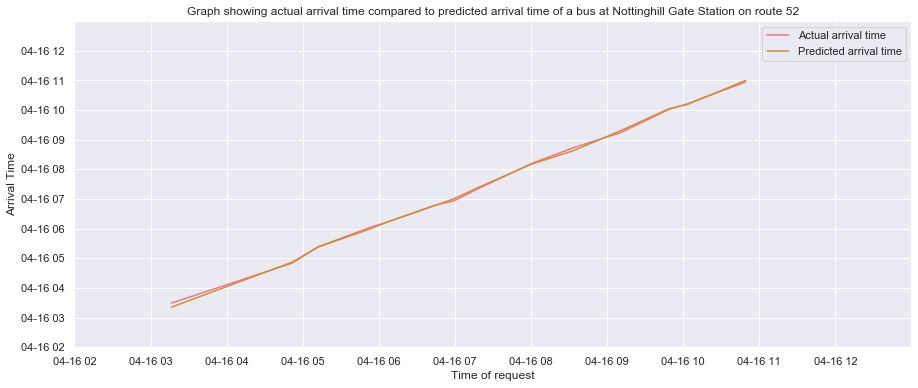
\includegraphics[keepaspectratio, width=15cm]{Images/historical-pred-actual-52.png}
    \caption{Bus 52}
    \label{fig:historical-pred-actual}
\end{center}
\end{figure}

\subsection{Regression Models}

\subsection{Neural Network Models}

\clearpage